%!TEX root = ../main.tex

\centerline{\textbf{\xiaoer{本科毕业论文外文翻译}}}
\bigskip

\noindent 文献原文:

\noindent Chen C, Zheng X, Wang Y, et al. Capturing Semantic Correlation for Item Recommendation in Tagging Systems[C]//AAAI. 2016: 108-114.

\vspace{1cm}


\centerline{\textbf{\sanhao{利用标签的语义关联性进行物品推荐}}}

\vspace{10pt}

\textbf{摘要}\quad
标签系统的普及对于提升物品推荐的效果是一个很好的机会。虽然现有的方法对标签使用主题建模来挖掘物品的语义信息,但是他们忽略了一个重要的性质,标签是用户和物品之间连接的桥梁。因此,这些方法不能处理无共同评分项的数据稀疏性问题(DS-WO-CRI),从而限制了它们的推荐性能。为了解决这个问题,我们提出了一种新型的基于标签和评分的协同过滤推荐模型,首先使用主题建模依次挖掘每个用户和每个物品的语义信息,然后将这些语义信息纳入矩阵分解,同时捕获标签和评分在用户和物品间的桥接特性。因此,我们的模型捕获了用户和物品间的语义关联,极大的提高了推荐性能,尤其是在 DS-WO-CRI 的情况下。在两个流行的真实数据集上的实验表明,我们提出的模型在准确率和召回率上显著优于传统的协同过滤方法、最先进的基于社交关系的协同过滤和基于主题模型的的协同过滤方法,它是解决 DS-WO-CRI 问题的有效方法。

\chapter{引言}
近些年来,诸如 Delicious(社交书签),Last.fm(社交音乐),Flickr(照片分享)和 YouTube(视频分享)这些标记系统为用户提供了高效的方式来组织、管理、共享并搜索各种项目。例如,一个人在 Last.fm 听 Lady Gaga 的音乐时,他可以将她标记为 “流行的” 和 “女歌手” 。这些连同评分行为一起出现的标签很有价值,强烈建议使用这样的信息来提供个性化推荐 \cite{Zheng2011A} 。

标签系统的普及促进了推荐系统的发展,尤其是标签系统中的协同过滤方法。目前为止,标签系统中主要有两种类型的协同过滤:标签推荐 \cite{Wang2013Collaborative} 的目的是为物品推荐合适的标签,另一种是基于标签的物品推荐 \cite{Zhou2009TagRec,Zhou2010UserRec},它关注利用标签和评分等信息为目标用户推荐相似的用户或物品。

目前,一个研究的趋势是在协同过滤中使用主题模型来处理标签信息 \cite{Agarwal2010fLDA,Wang2011Collaborative,purushotham2012collaborative,Wang2013Collaborative,Chen2014Context}。例如,Wang 和 Blei \cite{Wang2011Collaborative} 提出了一个协同主题回归(CTR)模型,可用于基于标签的物品推荐。Chen 等人 \cite{Chen2014Context} 提出的将 CTR 与社交矩阵分解 \cite{Ma2011Recommender} 结合的推荐方法获得了更好的预测效果。然而,这些方法只是将标签与用户和物品相关联,而忽略了标签重要性质,标签连接了用户和物品,这与评分的作用是一样的。但是标签可以反应用户和物品间的语义关联性,而评分没有这样的能力。

当一个用户为一些物品赋予了标签,那这些标签就反映了用户对物品的偏好。一个标签越频繁被一个用户使用,越可能表示这个用户喜欢这个标签所指代一类的物品\cite{Zheng2011A}。类似的,如果一个标签被越多的用户赋予一个物品,那么很可能这个物品匹配这个标签。因此,标签同时包含用户和物品的语义信息,而不仅仅是单独的用户或物品。

\textbf{一个针对性的例子}\quad 图 \ref{fig:fig1} 描述了一个标签系统的例子,这个系统包含三个用户($u_1, u_2, u_3​$),四个物品($v_1,v_2,v_3,v_4​$)和五个标签(“algorithm”, “journal”, “research”, “NBA”, “Kobe”)。

\begin{figure}
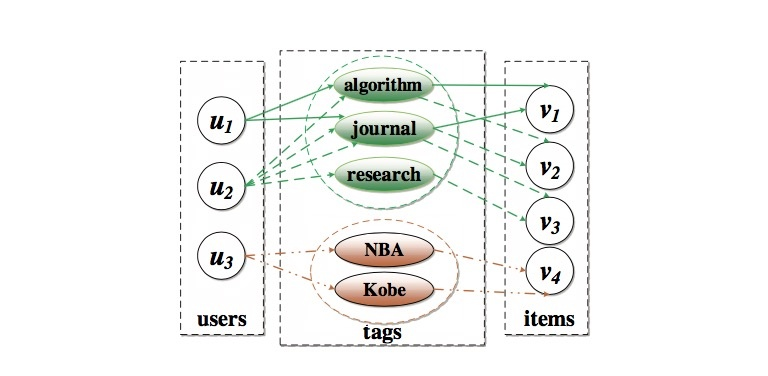
\includegraphics[width=\linewidth]{images/figure1.jpg}
\caption{一个标签系统的例子。每个标签都对应了一个评分,为简洁起见省略了评分。}
\label{fig:fig1}
\end{figure}


这个例子中,用户 $u_1$ 标注了物品 $v_1$,用户 $u_2$ 标注了物品 $v_2$ 和 $ v_3$,因此,用户 $u_1$ 和用户 $u_2$ 之间没有共同评分项。我们定义这种情况为*无共同评分项的稀疏性问题(DS-WO-CRI),DS-WO-CRI 是标准的数据稀疏性问题(在所有的用户物品对中只有很少比例的已知项)的一个典型子集。在 DS-WO-CRI 的情况下,已有的协同过滤方法,例如,PMF 和 CTR 模型,都无法将物品 $v_1$ 推荐给用户 $u_2$ ,因为这些方法无法捕获它们之间的任何联系。然而,一个好的推荐系统应该能够将物品 $v_2$ 和 $v_3$ 推荐给用户 $u_1$ 并且将物品 $v_1$ 推荐给用户 $u_2$,因为在这个例子中,用户 $u_1$ 和 $u_2$ 很可能是算法方面的研究者,而物品 $v_1$, $v_2$ 和 $v_3$ 可能跟算法有关。

现有的研究表明,用户对一个物品的评分或标注等动作就可以表明用户喜好该物品,而不需考虑评分的等级\cite{Koren2008Factorization,Koren2009Matrix}。换句话说,用户通过标记和评分隐式的表达了他的偏好\cite{Koren2008Factorization}。因此,一个用户和他所标注和评分的物品趋向于具有相似的潜在特征,我们在本文中将其定义为隐式偏好(implicit preference)。在上面的例子中,用户 $u_2$ 将物品 $v_3$ 标注为 “journal” 和 “research”,这在表明用户 $u_2$ 可能是一名研究者同时,也指出物品 $v_3$ 可能是一篇学术期刊或其他相关的东西。因此,在语义上,用户 $u_2$ 和物品 $v_3$ 的潜在特征应该具有某种程度的相似。

然而,现有的方法无法捕获用户和物品之间的语义关系,因此它们的推荐性能被局限了,尤其是在 DS-WO-CRI 的情况下。


\textbf{我们的提议}\quad 为了解决上面提到的 DS-WO-CRI 问题,我们在这篇文章中提出了一种新型的协同过滤系统。我们首先利用主题模型依次为每一个用户和每一个物品挖掘标签的语义信息,然后将这些语义信息纳入矩阵分解,同时捕获标签和评分在用户和物品间的桥接特性(即,隐式偏好)。因此,我们的模型可以捕获用户和项目间的语义关联,并将具有相似语义信息的物品推荐给用户,即便是在 DS-WO-CRI 的情况下。

\textbf{贡献}\quad 我们的工作主要有以下贡献:
(1)我们首先指出标签的重要特性,即它们做为桥梁将用户和物品连接起来,概述了用户和物品之间的语义联系,然后我们说明了利用此特性可以帮助解决 DS-WO-CRI 问题。据我们所知,这是首个针对这个问题的研究。
(2)我们提出了一种新型的基于标签和评分的协同过滤模型,它可以捕获用户和物品之间的语义联系,因此可以大大地提升推荐性能,尤其是在 DS-WO-CRI 的情况下。我们还提出了基于坐标上升的参数学习方法。据我们所知,这项研究是文献中对捕获用户和物品语义关联的首次尝试。
(3)在两个流行的真实世界的数据集上的实验表明,我们提出的模型在精确率和召回率方面都显著优于最先进的方法。实验还表明,我们的模型是一个解决 DS-WO-CRI 问题的有效方法。


\chapter{相关工作}
在本节中,我们将分三组来回顾已有的物品推荐方法,其中包括:传统的协同过滤方法、基于主题模型的协同过滤方法、以及基于社交关系的协同过滤方法。

基于已有的研究\cite{shi2014collaborative},传统的协同过滤方法仅利用用户物品的评分进行推荐,主要分为两种类型:基于内存的协同过滤\cite{deshpande2004item}和基于模型的协同过滤\cite{Koren2009Matrix,Koren2008Factorization,Zhou2009TagRec,Xu2015Ice},这两种方法都可以用于标签系统的推荐。

传统的协同过滤方法无法借助文本内容的信息,因此,一些混合模型被提出来,它们结合基于内容的方法和协同过滤方法进行推荐\cite{Melville2002Content}。但是,这些方法简单的将内容表示为词向量的形式,因而无法发掘它们的语义信息。为了利用内容所提供的语义信息,研究者利用主题模型提高推荐效果,Agarwal 等人提出了 fLDA 模型\cite{Agarwal2010fLDA},该方法通过将 LDA 中学习到的先验信息加入物品向量,结合了 RLFM\cite{Agarwal2010fLDA} 和隐式狄利克雷分布(LDA)。RLFM 和 fLDA 都能纳入额外的原信息,例如用户年龄和物品类别,然而,这些附加元特征信息不在本文的范围之内。稍后的,Wang 等人\cite{Wang2011Collaborative} 将概率矩阵分解\cite{Salakhutdinov2008Probabilistic} 与 LDA \cite{Blei2003Latent} 相结合,提出了协同主题回归模型。在\cite{Wang2011Collaborative} 中证明了在相似的情况下 CTR 的性能要优于 fLDA,因为 fLDA 基本忽略了其他用户的评分。

此外,用户之间和物品之间的社会信息对于提升推荐的性能是有效的\cite{Chen2013Recommender}。首先,用户的社会信息被纳入常规的协同过滤模型\cite{Jamali2010A},例如,Ma 等人提出 Soreg 来约束具有联系的用户的潜在因子之间的差异性。之后,相邻用户和物品的社会信息被引入了基于主题模型的协同过滤中以进一步改善推荐性能,例如,Purushotham、Liu 和Kuo \cite{purushotham2012collaborative} 以及 Chen 等人 \cite{Chen2014Context} 提出了两种模型(CTR-SMF 和 CTR-SMF2),将用户社交关系网络纳入CTR,以进一步提高项目推荐性能。Wang、Chen 和 Li \cite{Chen2014Context} 提出了一个将物品的社会关系引入 CTR 的模型,以提高标签系统中的标签推荐性能。


\chapter{提出的模型——TRCF}
在本节中,我们提出一个新的基于标签和评分的协同过滤方法(TRCF)。我们首先正式确定基于标签的物品推荐问题并定义一些符号。然后,我们提出 TRCF ,这是一个分层的贝叶斯模型。最后,我们提出了基于坐标上升的参数学习方法。

\section{初步定义}
假定,我们有一个用户的集合 $U=\{u_1,\dots,u_I \}$,这些用户用一组标签 $T=\{t_1,\dots,t_N \}$ 标记了的一组物品 $V=\{v_1,\dots,v_J \}$,以及评分的集合  $R=\{r_1,\dots,r_O \}$,其中,$I$ 、$J$、$N$ 和 $O$ 依次代表了用户、物品、标签和评分的数目。每一个用户-物品-标签-评分(U-I-T-R)的可观察数据是一个四元组$(u_i, v_j, T_{ij}, R_{ij})$,其中 $u_i \in U$,$v_j \in V$,$T_{ij}$ 是用户 $u_i$ 给予物品 $v_j$ 的标签集合,并且 $T_{ij} \in T$ ,$R_{ij}$ 是用户 $u_i$ 给予物品 $v_j$ 的评分,评分基于用户对该物品的喜好程度并在同时标注它。然而,用户-物品(U-I)的评分集合 $R$ 一般是整数集合,例如,*MovieLens* 使用 [1,5] 范围内的评分。$U \in R^{K*I}$ 表示潜在的用户特征矩阵,其中列向量 $U_i$ 表示属于用户 $u_i$ 的 $K$ 维潜在特征向量。$V \in T^{K*J}$ 表示潜在的物品特征矩阵,其中列向量 $V_j$ 表示属于物品 $v_i$ 的 $K$ 维潜在特征向量。

对于基于标签和评分的物品推荐中,给定现有的四元组 U-I-T-R ,我们的目标是预测用户 $u_i$ 对物品 $v_j$ 的未知的评分。

\section{基于标签和评分的协同过滤}
TRCF 是一个新型的分层的贝叶斯模型,图 \ref{fig:fig2} 展示了它的图模型,其中 $N_u$ 和 $N_v$ 依次表示用户 $u_i$ 和物品 $v_j$ 的标签数目。我们首先将每个用户和物品的标签依次分组,然后使用隐式狄利克雷分布依次对每个用户和每个物品的标签集合进行语义挖掘(图 \ref{fig:fig2} 中以红色绘制)。最后将这些语义信息纳入矩阵分解用于分解评分信息(图 \ref{fig:fig2} 中以紫色绘制)以及捕获标签和评分所提供的隐式偏好(图 \ref{fig:fig2} 中以蓝色绘制)。
\begin{figure}
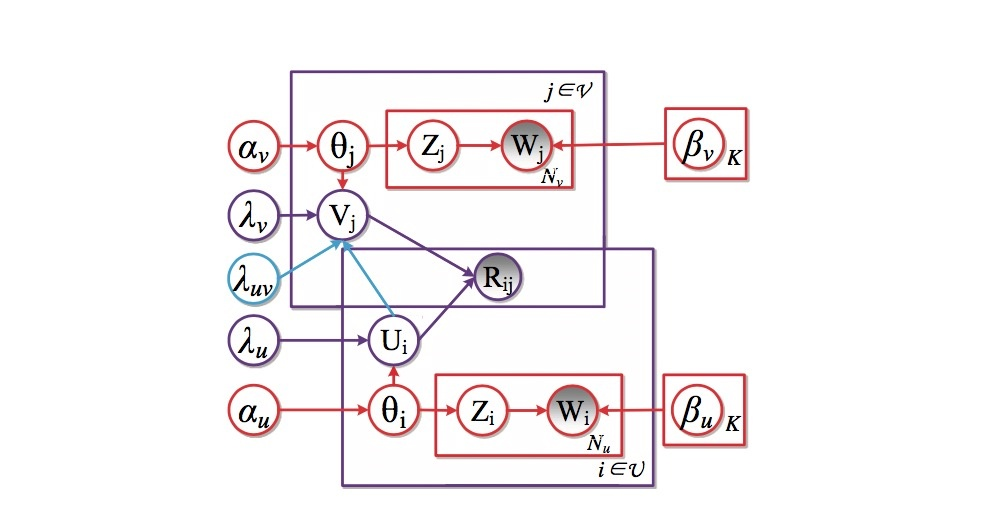
\includegraphics[width=\linewidth]{images/figure2.jpg}
\caption{TRCF 的图模型。LDA 部分以红色绘制,隐式偏好部分以蓝色绘制,PMF 部分以紫色绘制。}
\label{fig:fig2}
\end{figure}

TRCF 同时在用户和物品两个方面上执行 LDA ,因此可以同时捕获用户和物品的语义信息,而不仅仅像现有的工作那样只捕获物品的语义信息。另外,在 TRCF 中,如果一个用户和一个物品通过标签或评分相关联,那么他们的隐式特征会在某些程度上比较相似,这被称为隐式偏好。相比之下,现有的基于主题建模的CF方法,例如,CTR、CTR-SMF 和 CTR-SMF2,都是假设用户和物品是独立的,并且忽略标签和评分在用户和项目之间的桥接作用。因此,TRCF 可以捕获用户和物品之间的语义关联,并且能够处理 DS-WO-CRI 问题。假定每个用户和每个物品都有 $K$ 个主题, TRCF 的执行过程如下:

\begin{enumerate}[itemindent=1em]
	\item \textbf{挖掘用户标签的语义信息。} 对于每个用户 $u_i$ :
	\begin{enumerate}[itemindent=1em]
		\item 选取主题分布 $\theta_i \sim Dirichlet(\alpha_u)$ ;
		\item 选取用户的潜在向量 $U_i \sim \mathcal{N}(\theta_i, \lambda_u^{-1} I_k)$ ;
		\item 对于用户 $u_i$ 的每一个标签 $w_{in_u}$ :
		\begin{enumerate}[itemindent=1em]
			\item 选取主题 $z_{in_u} \sim Mult(\theta_i)$ ;
			\item 选取标签 $w_{in_u} \sim Mult(\beta_{z_{in_u}}) $ ;
		\end{enumerate}
	\end{enumerate}
	\item \textbf{挖掘物品标签的语义信息,并且采集用户和物品间的隐式偏好。} 对于每一个物品 $v_j$ :
	\begin{enumerate}[itemindent=1em]
		\item 选取主题分布 $\theta_j \sim Dirichlet(\alpha_v)$ ;
		\item 选取物品的潜在向量 $V_j \sim \mathcal{N}(\theta_j, \lambda_v^{-1} I_k) \times \prod\limits_{i} I_{ij}^R \mathcal{N}(U_i, \lambda_{uv}^{-1}I_K ) $ ;
		\item 对于物品 $v_j$ 的每一个标签 $w_{jn_v}$ :
		\begin{enumerate}[itemindent=1em]
			\item 选取主题 $z_{jn_v} \sim Mult(\theta_j)$ ;
			\item 选取标签 $w_{jn_v} \sim Mult(\beta_{z_{jn_v}}) $ ;
		\end{enumerate}
	\end{enumerate}
	\item \textbf{获取评分。} 对于每一个用户-物品对 $(i,j)$ :
	$$
		R_{ij} \sim \mathcal(U_i^ T V_j, c_{ij}^{-1}).
	$$
\end{enumerate}

在上面的生成过程中,$\mathcal{N} \sim (x | \mu, \sigma^2)$ 是期望为 $\mu$ 方差为 $\sigma^2$ 的高斯分布,$I_K$ 是一个 $K$ 行 $K$ 列的单位矩阵。$I_{ij}^R$ 是一个指示函数,如果用户 $u_i$ 为物品 $v_j$ 打分了,它的值为 1,否则为 0。$C$ 是评分置信度矩阵,其中的项 $c_{ij}$ 表示评分的置信度。更多细节请参考\cite{Wang2011Collaborative}。

参数 $\lambda_u$ 平衡了用户语义信息提供的标签和评分信息对模型性能的影响。类似地,参数 $\lambda_v$ 平衡了由物品语义信息提供的标签和评分信息对推荐性能的影响。参数 $\lambda_{uv}$ 平衡隐式偏好对模型性能的贡献,即通过评级和标签链接的用户和项目之前潜在特征相似度的程度。

观察到的评分的条件分布可以被形式化为:
$$
p(R | U, V, C) = \prod\limits_i \prod\limits_j \mathcal{N} (R_{ij}|U_i^T V_j,c_{ij}).
$$

用户和物品的潜在向量 $U_i$ 和 $V_j$ 生成的方式与 CTR 相似,它们可以被形式化为:
\begin{equation}
\begin{aligned}
&p(U|\lambda_u) \sim \prod\limits_i \mathcal{N} (\theta_i, \lambda_u^{-1}I_K), \\
&p(V|U, \lambda_v, \lambda_{uv}) \sim  \prod\limits_j \mathcal{N} (\theta_j, \lambda_v^{-1}I_K)  \times \prod\limits_{i} I_{ij}^R \mathcal{N}(U_i, \lambda_{uv}^{-1}I_K ).
\end{aligned}
\end{equation}

给定了 U-I-T-R 信息,通过使用贝叶斯推理,我们可以得到 TRCF 的潜在特征向量的后验概率的如下式子:
\begin{equation}
p(U,V| R,C,\lambda_u, \lambda_v, \lambda_{uv})  \propto p(R | U, V, C) p(U|\lambda_u) p(V|U, \lambda_v, \lambda_{uv}) .  
\label{eq1}
\tag{1}
\end{equation}


\section{TRCF 的参数学习}

给定主体参数 $\beta_u$ 和 $\beta_v$ ,直接计算 $U_i, V_j, \theta_i, \theta_j$ 的完整后验是困难的。我们使用坐标上升的方法来学习最大后验概率。使等式 $\eqref{eq1}$ 中具有固定超参数的两个潜在特征的后验最大化等价于,在给定 $\lambda_u , \lambda_v$ 的条件下, 使如下的 $U, V, \theta_{1:I}, \theta_{1:J}$ 的对数似然函数最大:
\begin{equation}  
\begin{aligned}
L = & -\frac{\lambda_u}{2} \sum\limits_i{ (U_i - \theta_i)^T  (U_i - \theta_i) }  \\ 
	& -\frac{\lambda_v}{2} \sum\limits_j{ (V_j - \theta_j)^T  (V_j - \theta_j)   } \\
	& -\sum\limits_{ij} \frac{c_{ij}}{2} (R_{ij} - U_i^T V_j)^2 \\
	& +\sum\limits_i \sum\limits_{n_u} log \left(\sum\limits_k \theta_{ik} \beta_{k,w_{in_u}} \right) \\
	& +\sum\limits_j \sum\limits_{n_v} log \left(\sum\limits_k \theta_{jk} \beta_{k,w_{jn_v}} \right) \\
	& - -\frac{\lambda_{uv}}{2} I_{ij}^R \sum\limits_{ij} (U_i - V_j)^T (U_i - V_j).  
\end{aligned} 
\label{eq2}
\tag{2}
\end{equation}

我们省略一个常数并设置狄利克雷先验 $\alpha_u = \alpha_v = 1$ 。这个函数可以通过使用坐标上升来优化,也就是说,我们固定 $\beta_u$ 和 $\beta_v$ ,并迭代优化 MF 变量 $U_i , V_j$ 和主题分布 $\theta_i , \theta_j$ 。具体来说,我们首先根据 $\theta_i , \theta_j$ 当前的估计值更新 $U_i$ 和 $V_j$ ,我们计算等式 $\eqref{eq2}$ 中 $L$ 在 $U_i , V_j$  上的导数,并且将它设置为 0 :
\begin{equation}
\label{eq3}
\frac{\partial{L}}{\partial{U_i}}  = 0, \frac{\partial{L}}{\partial{V_j}}  = 0.
\tag{3}
\end{equation}

解决上述的公式得到参数更新的式子:
\begin{equation}  
\begin{aligned}
& U \leftarrow  \left(  VC_iV^T + \lambda_uI_K  + \lambda_{uv}\sum\limits_i I_{ij}^R I_K \right)^{-1}
(VC_iR_i + \lambda_u\theta_i + \lambda_{uv} \sum\limits_j {I_{ij}^R V_j}), \\
& V \leftarrow  \left(  UC_jU^T + \lambda_vI_K  + \lambda_{uv}\sum\limits_i I_{ij}^R I_K \right)^{-1}
(UC_jR_j + \lambda_v\theta_j + \lambda_{uv} \sum\limits_i {I_{ij}^R U_i}).
\end{aligned} 
\label{eq4}
\tag{4}
\end{equation}

其中对于每一个用户 $u_i$ ,$C_i$ 是一个对角矩阵,它的对角元素是 $c_{ij}, j= 1, \dots, J$ ,并且 $R_i = {R_{ij}} _{j=1}^J$ 。对于物品 $v_j$ ,$C_j$ 和 $R_j$ 的定义是相似的。

公式 $\eqref{eq4}$ 显示了参数 $\lambda_u$、$\lambda_v$ 和 $\lambda_{uv}$ 是如何影响用户和物品的潜在特征的。越大的 $\lambda_u$ 会导致用户的潜在特征越依赖于用户标签,而不是评分信息。类似的,较大的 $\lambda_v$ 表示物品的潜在特征来自物品标签的比例更大,而不是评分信息。此外,更大的 $\lambda_{uv}$ 意味着更强的约束,即通过标签和评分链接的用户和项目应当具有类似的潜在特征,即隐式偏好。从公式 $\eqref{eq4}$ 可以看出,概率矩阵分解(PMF)和协同主题回归(CTR)都是 TRCF 的特殊形式。

接下来,给定当前的 MF 变量 $U_i , V_j$ ,我们更新主题分布参数 $\theta_i$ 和 $\theta_j$ 。对于 $\theta_i$ ,我们先定义 $q(z_{in_u} = k) = \phi_{in_uk}$ ,然后分离包含 $\theta_i$ 的用户并应用 Jensen 不等式:
\begin{equation}  
\begin{aligned}
L(\theta_i) &\geq -\frac{\lambda_u}{2}  (U_i - \theta_i)^T  (U_i - \theta_i)  \\
& + \sum\limits_{n_u} \sum\limits_k{ \phi_{in_uk} (log{\theta_{ik} \beta_{k, w_{in_u}}  -  log{\phi_{in_uk}} })}  \\
&=L(\theta_i, \phi_i).
\end{aligned} 
\end{equation}

其中,$\phi_i = {\phi_{in_uk}}_{n_u=1,k=1}^{N_u \times K}$ 。显然 $L(\theta_i, \phi_i)$ 是 $L(\theta_i)$ 的严格下界,因此我们可以使用映射梯度\cite{bertsekas1999nonlinear} 来优化 $\theta_i$ 。最优的 $\phi_{in_uk}$ 正比于 $\theta_{ik} \beta_{k,w_{in_u}}$ 。对于 $\theta_j$ ,更新的规则是相似的。

对于 $\beta_u$ ,我们像 LDA 那样为主题执行 M 步的更新。
$$
\beta_{kw_i} \propto \sum\limits_i \sum\limits_{n_u} \phi_{in_uk} 1 [w_{in_u} = w].
$$

对于 $\beta_v$ ,它的更新策略是相似的。当参数 $U^*, V^*, {\theta_{1:I}}^*,  {\theta_{1:J}}^* , {\beta_u}^*, {\beta_v}^*$ 的最优值学习完成后,我们的模型就可以进行评分预测了:
$$
{R_{ij}}^* \approx ({U_i^*})^T V_j^*.
$$


\chapter{实验和分析}
在本节中,我们介绍了对两个流行的现实世界数据集进行的实验,目的是回答如下的问题:(1)我们的模型相比现有的最先进的方法有什么改进? (2)我们的方法如何处理 DS-WO-CRI 问题? (3)参数 $\lambda_u$ ,$\lambda_v$ 和 $\lambda_{uv}$ 如何影响 TRCF 的性能?

\section{数据集}
我们在实验中使用了两个现实世界的数据集:hetrec2011-delicious-2k (Delicious) 和 hetrec2011-lastfm-2k (Lastfm)\cite{Cantador2011Second}。这两个数据集已广泛用于标签系统的实验\cite{Bellog2013A},它们在表 \ref{table1} 中描述。

\begin{table}[]
\centering
\caption{数据集描述}
\label{table1}
\begin{tabular}{@{}cccccc@{}}
\toprule
数据集       & 用户   & 物品    & 标签    & 用户-标签-物品 & 评分     \\ \midrule
Delicious & 1867 & 69226 & 53388 & 437593   & 104799 \\
LastFm    & 1892 & 17632 & 11946 & 186479   & 92834  \\ \bottomrule
\end{tabular}
\end{table}

对于每个数据集,如果用户已将该项目设为书签(或收听),则我们认为该项目的用户评分为 1 ,否则,该项目的用户评分为 0 。

在我们的实验中,我们将每个数据集分为三个部分——训练数据集(80%),留出验证数据集(10%)和测试数据集(10%)。 我们在训练数据集上训练我们的模型,在验证数据集上获得最佳参数,并在测试数据集上评估我们的模型。

\section{比较与评估}
如相关工作中所述,存在许多种推荐方法,例如,基于存储的方法和混合方法。这里,我们将所提出的 TRCF 与以下三种现有的方法进行比较,即常规的协同过滤方法,基于社会关系的 CF 方法和基于主题建模的方法:

% \begin{enumerate}[itemindent=1em]
% \item SVD ++(Koren, 2008)是一种经典的协同过滤方法,该方法仅使用 U-I 评分信息。
% \item Soreg(Ma et al., 2011)是基于社会关系的 CF 方法,其使用 U-I 评分和用户社交信息。
% \item CTR (Wang and Blei, 2011)是一种最先进的基于主题建模的 CF 方法,其使用类似于 TRCF 中使用的四元组 U-I-T-R 的信息。
% \item CTR-SMF(Purushotham, Liu, and Kuo, 2012)结合了用户社交矩阵分解和 CTR 。 它包含除了在 TRCF 中使用的四元组 U-I-T-R 之外的附加用户社交信息。
% \item CTR-SMF2(Chen et al., 2014)改进了 CTR-SMF ,它还将用户社交信息引入了 TRCF 中的 U-I-T-R 四元组。
% \end{enumerate}

\textbf{SVD ++} \cite{Koren2008Factorization} 是一种经典的协同过滤方法,该方法仅使用 U-I 评分信息。

\textbf{Soreg} \cite{Ma2011Recommender} 是基于社会关系的 CF 方法,其使用 U-I 评分和用户社交信息。

\textbf{CTR} \cite{Wang2011Collaborative} 是一种最先进的基于主题建模的 CF 方法,其使用类似于 TRCF 中使用的四元组 U-I-T-R 的信息。

\textbf{CTR-SMF} \cite{purushotham2012collaborative} 结合了用户社交矩阵分解和 CTR 。 它包含除了在 TRCF 中使用的四元组 U-I-T-R 之外的附加用户社交信息。

\textbf{CTR-SMF2} \cite{Chen2014Context} 改进了 CTR-SMF ,它还将用户社交信息引入了 TRCF 中的 U-I-T-R 四元组。

精确率和召回率已被广泛用作评估推荐效果的指标\cite{herlocker2004evaluating}。 因此,我们使用 Precision 和 Recall 来评估推荐性能,并且计算召回率的方式也用于 CTR,CTR-SMF 和 CTR-SMF2。 对于每个用户,Precision 和 Recall 定义如下:
\begin{equation}
\begin{aligned}
Precision@M = \frac{\# \text{Top M 中用户喜欢的物品}}{M},  \\
Recall@M = \frac{\# \text{Top M 中用户喜欢的物品}} {\# \text{用户喜欢的所有物品}}, 
\end{aligned}
\end{equation}
其中 M 是推荐列表中的物品数。 我们计算测试数据集中所有项的精确率和召回率的平均值作为最终结果。

\section{性能对比和分析}
在对比不同模型时,我们使用在 CTR-SMF \cite{purushotham2012collaborative} 中设置的 SVD++、CTR 和 CTR-SMF 的最佳参数,它们使用相同的数据集。 对于 Soreg、CTR-SMF2 和我们的模型,我们使用网格搜索来获得最佳参数。
\begin{figure}
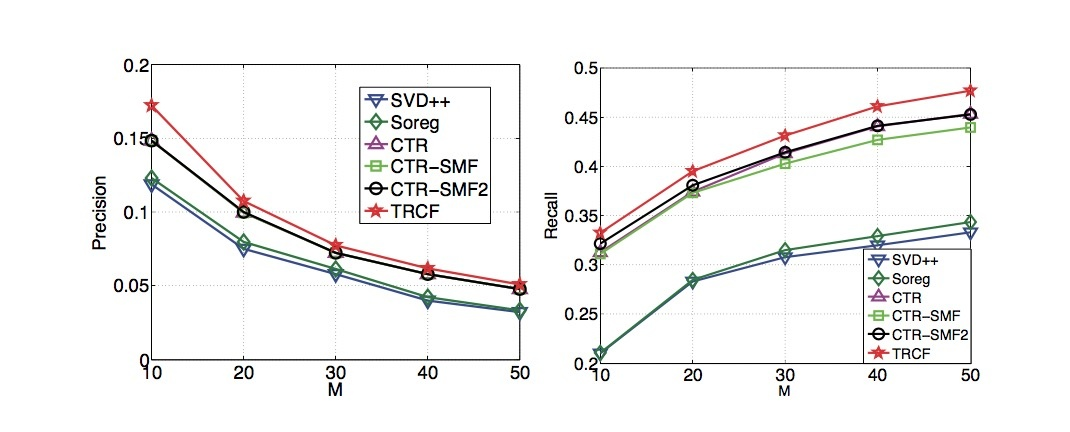
\includegraphics[width=\linewidth]{images/figure3.jpg}
\caption{在 Delicious 数据集下设置不同的 M 值,精确率和召回率的对比,以及每个方法的最优参数}
\label{fig:fig3}
\end{figure}
\begin{figure}
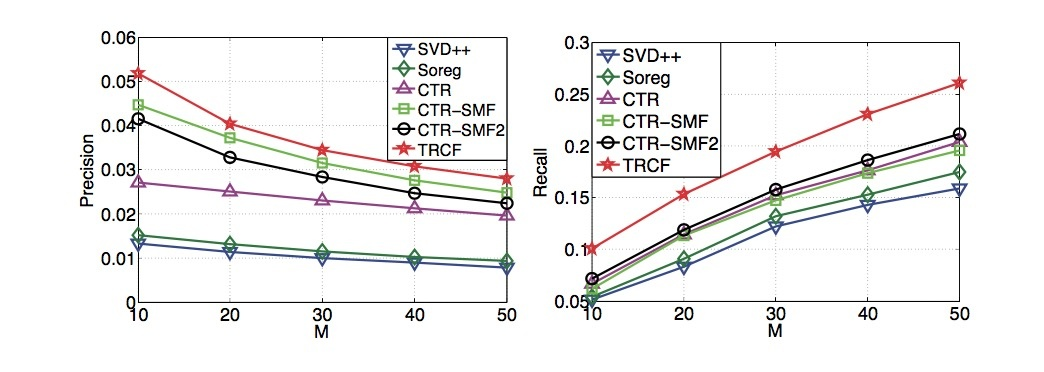
\includegraphics[width=\linewidth]{images/figure4.jpg}
\caption{在 LastFm 数据集下设置不同的 M 值,精确率和召回率的对比,以及每个方法的最优参数}
\label{fig:fig4}
\end{figure}


\textbf{结果:} 图 \ref{fig:fig3} 和图 \ref{fig:fig4} 显示了各个推荐方法在 Delicious 数据集和 Lastfm 数据集上的总体性能,其中我们设置 $M = 10,20,30,40,50$ 并将每个方法的参数固定为最佳值。 结果表明,传统的 CF 方法(SVD ++)和基于社交关系的 CF 方法(即 Soreg)具有相似的性能。 三个基于主题建模的 CF 方法(即 CTR、CTR-SMF 和 CTR-SMF2)具有类似的性能,并且显著优于 SVD++ 和 Soreg,这表明了标签信息在推荐中的重要性。

我们提出的 TRCF 方法在这两个数据集上显著优于 SVD++、Soreg、CTR、CTR-SMF 和 CTR-SMF2。具体在平均值上,在 Delicious 数据集上,TRCF 在精确度方面将 SVD++、Soreg、CTR、CTR-SMF 和 CTR-SMF2 提升了 46.75%、39.74%、8.62%、8.78% 和 8.65%,并且在召回率方面分别提高了 44.99%、42.40%、5.23%、7.27% 和 4.21% 。在 Lastfm 数据集上,TRCF 在精确度方面将 SVD++、Soreg、CTR、CTR-SMF 和 CTR-SMF2 提升了 259.80%、210.27%、57.96%、11.64% 和 23.85% ,并且在召回率方面分别提高了 73.03%、60.39%、34.18%、39.04% 和 28.12% 。


\textbf{分析和总结:} 以上的对比表明了我们提出模型的有效性,它捕获了用户和物品之间的语义关联。实验结果表明,尽管用户的社交信息可以改善推荐性能,但是改善推荐性能的更有效的方式是考虑用户和物品的语义相关性。


\section{DS-WO-CRI 实验}
所有四种基于主题建模的 CF 方法(包括 TRCF)都可以通过采集物品的语义信息来提高推荐性能。为了研究它们处理 DS-WO-CRI 问题的能力,我们进行以下实验。我们首先依据 DS-WO-CRI 的程度将 LastFm 数据集分为四个子数据集,每个数据集在表 2 中描述了。DS-WO-CRI 的程度定义如下:
$$
x\% = \frac{\#\text{没有共同评分物品的用户数目}}{\#\text{总的用户数目}}.
$$
然后我们对每个子数据集进行对照实验。图 \ref{fig:fig5} 显示,我们的模型在不同的 DS-WO-CRI 程度下都达到最佳性能。我们的模型相对于其他三个主题建模方法的在 LC1、LC2、LC3、LC4 上精确率的平均改进分别为 49.67%、75.81%、345.77% 和 428.97% ,召回率的改进分别为 33.94%、65.00%、383.63 % 和 458.00% 。实验结果表明,DS-WO-CRI 的程度越严重,我们的模型相对其它模型的优势越明显。
\begin{figure}
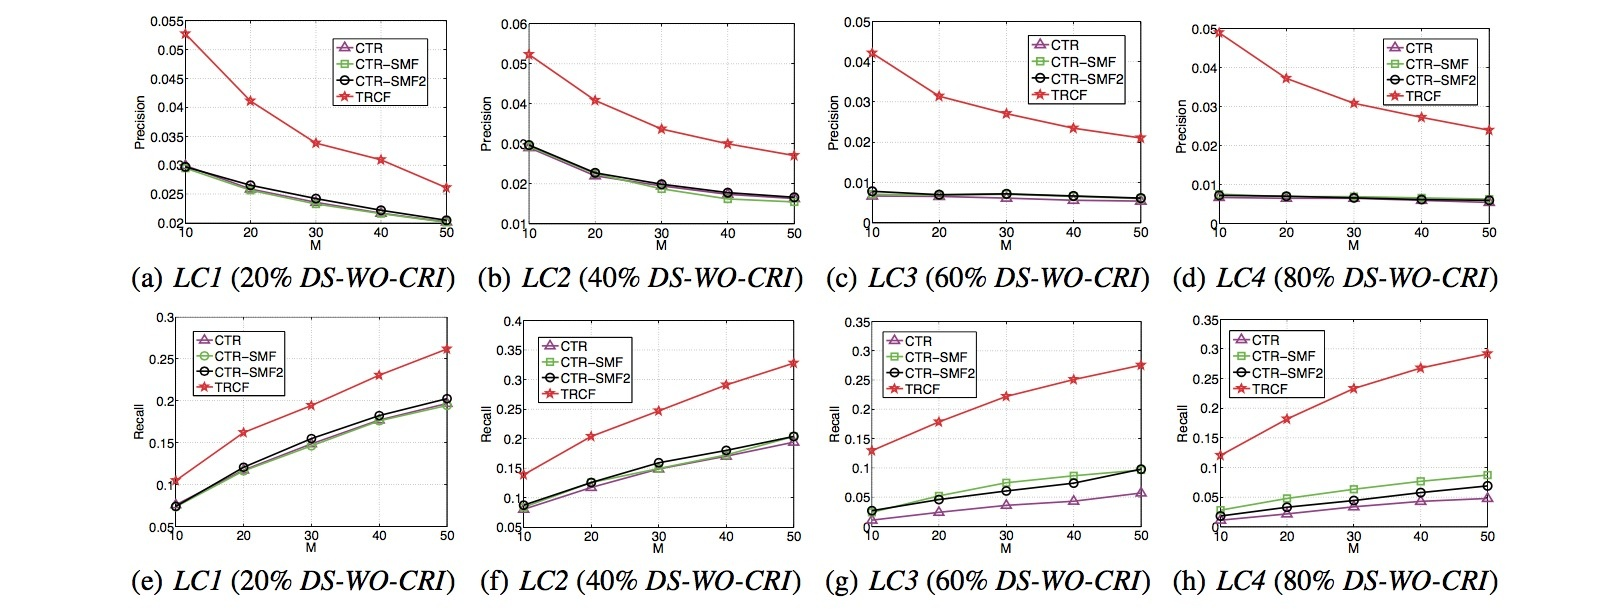
\includegraphics[width=\linewidth]{images/figure5.jpg}
\caption{在每个 DS-WO-CRI 子数据集上设置每种方法的最优参数,精确率和召回率对比。}
\label{fig:fig5}
\end{figure}

\textbf{总结:} DS-WO-CRI 实验表明了我们提出的模型在处理该问题时的有效性:越严重的 DS-WO-CRI 情况,我们的模型相比其它模型的优势越明显。这是由于我们的方法具有采集用户和物品间标签语义关联的能力。


\section{参数影响}
图 \ref{fig:fig6:a} 显示了在 LastFm 数据集上固定公式 $\eqref{eq2}$ 中的参数 $\lambda_{uv} $ 时, 参数 $\lambda_u$ 和 $\lambda_v$ 对 TRCF 性能的影响。我们可以看到,当 $\lambda_u = \lambda_v = 10$ 时,TRCF 达到最佳性能,这说明用户和物品语义信息都对模型性能有显着的贡献。图 \ref{fig:fig6:b} 显示了在四个 DS-WO-CRI 子数据集上固定 $\lambda_u$ 和 $\lambda_v$ 为最佳值时,公式 $\eqref{eq2}$ 中的参数 $\lambda_{uv} $ 对 TRCF 性能的影响。我们可以看到,TRCF 的性能首先随着 $\lambda_{uv} $ 的增大而上升,然后在某个阈值后开始下降。在 LC1、LC2、LC3、LC4 上最佳的 $\lambda_{uv}$ 值分别是 0.0001、0.01、0.01 和 0.1。这个结果说明了 DS-WO-CRI 的程度越大,对应的 $\lambda_{uv}$ 的最优值相应的越大。换句话来说,当 DS-WO-CRI 的问题越严重时,通过标签和评分(即隐式偏好)桥接用户和物品的特性越重要,这就解释了为什么我们的模型在可以在严重的 DS-WO-CRI 的情况下表现良好的原因。


\begin{figure}
\centering
\subfigure[$\lambda_u, \lambda_v$ 的影响]{
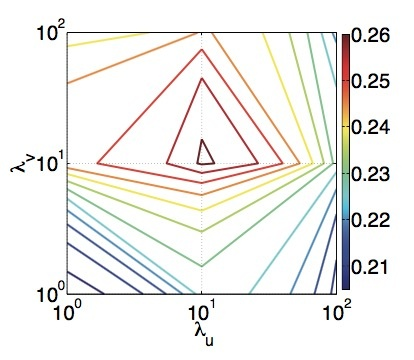
\includegraphics[width=0.45\linewidth]{images/figure6a.jpg}
\label{fig:fig6:a}
}
\subfigure[$\lambda_{uv}$ 的影响]{
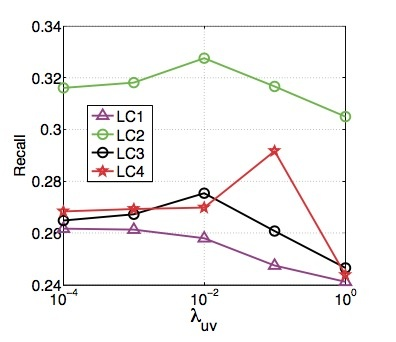
\includegraphics[width=0.45\linewidth]{images/figure6b.jpg}
\label{fig:fig6:b}
}
\caption{固定 M=50, $\lambda_u, \lambda_v, \lambda_{uv}$ 对 TRCF 召回率的影响。}
\end{figure}



\chapter{总结}
在本文中,我们首先介绍了在实际的标记系统中存在的 DS-WO-CRI 问题。 然后,我们提出一个新型的基于标签和评分的 CF 模型来处理这个问题。该模型使用主题建模来分别挖掘用户和物品的标签的语义信息,并将语义信息结合到矩阵分解中以对评分信息进行因式分解,并捕获用户与物品之间的标签和评分的桥接特征 。据我们所知,这是文献中首次尝试引入 DS-WO-CRI 问题并提出一个处理它的模型。 最后,对两个流行的数据集进行的实验表明,我们的模型在精确率和召回率方面显着优于目前最先进的方法,特别是在 DS-WO-CRI 情况下。

\chapter{致谢}
我们感谢匿名审稿人的有益建议。这项工作得到了中国国家自然科学基金(61379034)、国家重点技术研发计划(2014BAH28F05)、广东省科技计划(2013B040100004, 2013B040403002)和中国浙江省自然科学基金(LQ14F010006)的部分支持。


\bibliography{data/文献翻译}






